% Appendix1 file from standard thesis template
\appendixtitle
\appendix
\chapter{Source code}

The following is the source code to several programs that make the radiometer possible.  The first is the Python code used with the Ettus N200 software defined radio.  This code is a heir block, which means it can be imported into GNURadio and used as a block.  This python code should work on any platform that has the GNURadio libraries installed and also the USRP drivers for communicating with the N200.  Other SDRs and other source blocks can be used as well, just replace the USRP source with the source you intend to use.  This code can also be easily modified to communicate with any SDR that GNURadio can communicate with.  This code was generated using GNURadio Companion.  

The second code is the Matlab script that can be used to parse the output from GNURadio.  This code will plot the total power output as well as perform some other functions such as a NE$\delta$T calculation and also allows for calibration points to be entered as well.  This code can be used as a foundation for other programs.  

The third code supplied is Python code that can be used to read the data generated and plot it.  In many ways it mimics the functions of the Matlab script buy uses Python, NumPy and SciPy to perform the mathematical functions.  This may be a better option for those that wish to look at the data but do not have access to Matlab since Python is free to download.

Finally, this code has been included in this thesis as a point of reference.  It may be out of date and some other pieces of code was also used for the experimentation used in this thesis.  Copies of this thesis source \LaTeX code, and any other code used can be found on the author's GitHub repository, \url{https://github.com/matgyver/Radiometer-SDR-Thesis}.


\section*{Python code for total power radiometer}
The main code that acts as the total power radiometer is the TPR.py code.  This module adds a custom block to GRC that can then be called and used like any other block in GRC.  A screenshot of the blocks used in this is shown below.

{\begin{figure}[h!tb] 
\centering
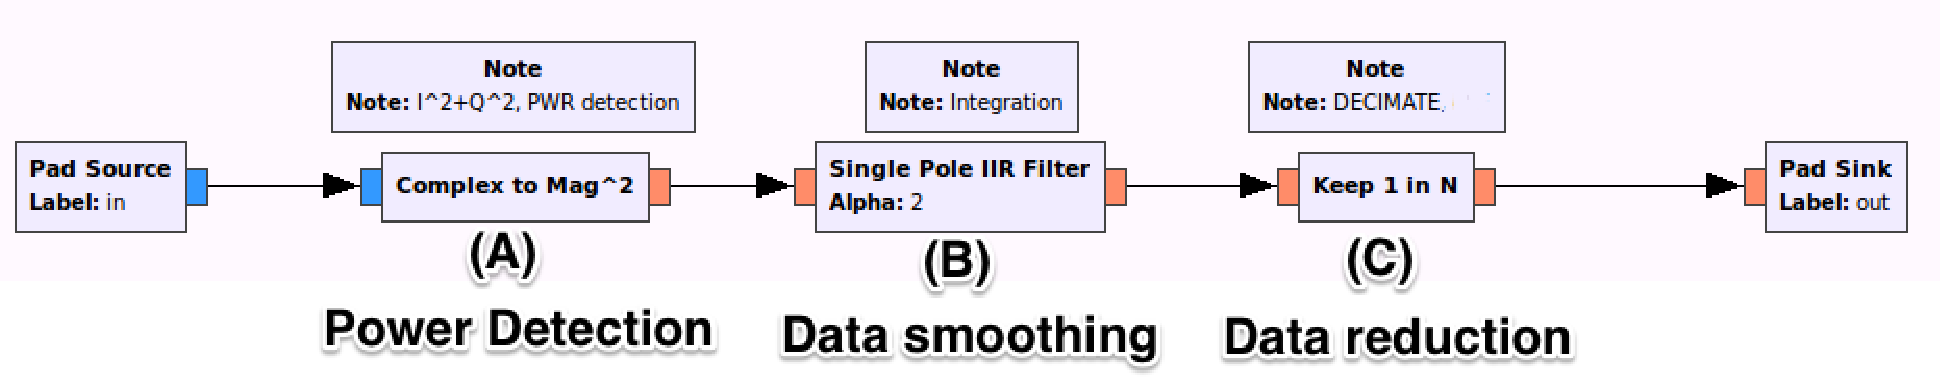
\includegraphics[width=0.8\linewidth]{Images/TPR_grc.png}
\isucaption{Blocks used for creating a total power radiometer in software}
\label{TPR_GRC}
\end{figure}
}
\lstset{
  language=Python,
  showstringspaces=false,
  formfeed=\newpage,
  tabsize=4,
  commentstyle=\itshape,
  basicstyle=\ttfamily,
  breaklines=true,
  morekeywords={models, lambda, forms}
}

\newcommand{\code}[2]{
  \hrulefill
  \subsection*{#1}
  \lstinputlisting{#2}
  \vspace{2em}
}

\code{Total Power Radiometer Block}{Code/TPR.py}
\newpage

\section*{Matlab code for reading and displaying data from GNURadio}
\lstset{
  language=Matlab,
  showstringspaces=false,
  formfeed=\newpage,
  tabsize=4,
  commentstyle=\itshape,
  basicstyle=\ttfamily,
  morekeywords={models, lambda, forms}
}

\newcommand{\matlabcode}[2]{
  \hrulefill
  \subsection*{#1}
  \lstinputlisting{#2}
  \vspace{2em}
}

\matlabcode{GNURadio Parsing Code}{Code/gnuradio_parse.m}
\newpage

\section*{Python code for analyzing data}
\lstset{
  language=Python,
  showstringspaces=false,
  formfeed=\newpage,
  tabsize=4,
  commentstyle=\itshape,
  basicstyle=\ttfamily,
  morekeywords={models, lambda, forms}
}

\newcommand{\pythoncode}[2]{
  \hrulefill
  \subsection*{#1}
  \lstinputlisting{#2}
  \vspace{2em}
}

\pythoncode{Total Power Radiometer}{Code/iPython/Radiometer_Parse.py}
\newpage